\documentclass[MASTER.tex]{subfiles} 
\begin{document} 
	
	
	\begin{frame}
		\huge
		\[ \mbox{Machine Learning with Python} \]
	\end{frame}
	
	%===========================================================%%=======================================================================%
\begin{frame}
\Large
\textbf{MachineLearning}

Machine Learning is a discipline involving algorithms designed to find patterns in and make predictions about data. It is nearly ubiquitous in our world today, and used in everything from web searches to financial forecasts to studies of the nature of the Universe. This tutorial will offer an introduction to scikit-learn, a python machine learning package, and to the central concepts of Machine Learning. 

\end{frame}
%=======================================================================%
\begin{frame}
\Large	\textbf{MachineLearning}
	We will introduce the basic categories of learning problems and how to implement them using scikit-learn. From this foundation, we will explore practical examples of machine learning using real-world data, from handwriting analysis to automated classification of astronomical images.

\end{frame}
%=======================================================================%
\begin{frame}[fragile]
\textbf{Getting ready}
The datasets in scikit-learn are contained within the datasets module. Use the following
command to import these datasets:
\begin{framed}
\begin{verbatim}
>>> from sklearn import datasets
>>> import numpy as np
\end{verbatim}
\end{framed}

\end{frame}
%======================================================================== %
\begin{frame}
	\begin{figure}
\centering
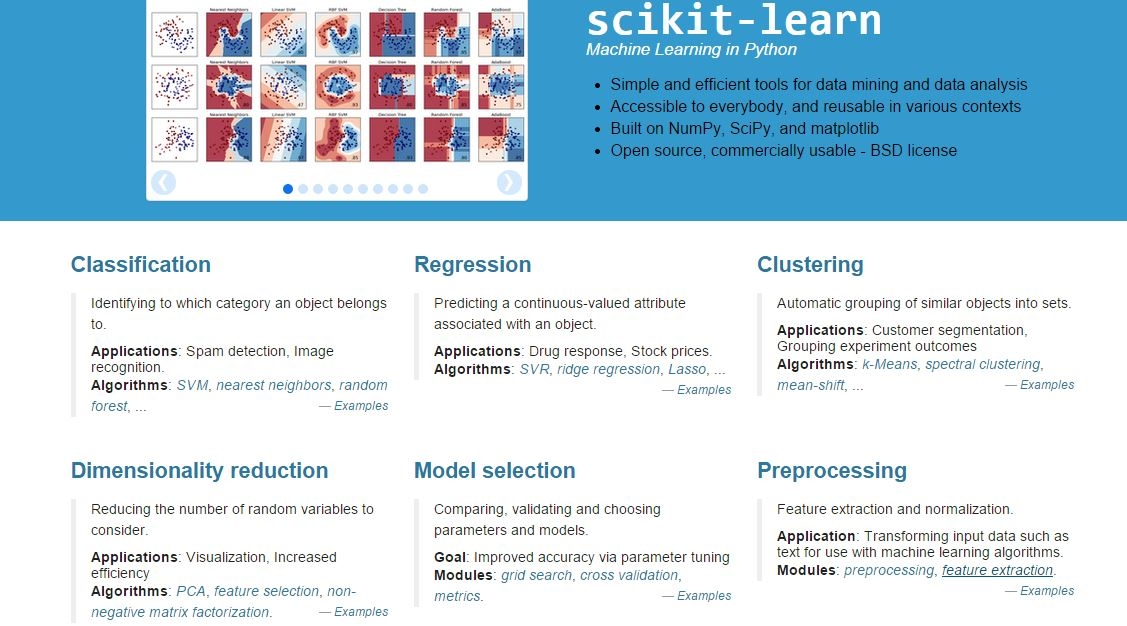
\includegraphics[width=1.2\linewidth]{SKLsite}

\end{figure}

\end{frame}
%=======================================================================%
\begin{frame}
	\LARGE
\textbf{Classification}
\begin{itemize}
\item \textbf{Description:} Identifying to which category an object belongs to.
\item \textbf{Applications:} Spam detection, Image recognition.
\item \textbf{Algorithms:} SVM, nearest neighbors, random forest, 
\end{itemize}

\end{frame}
%=======================================================================%
\begin{frame}
\LARGE
\textbf{Regression}
\begin{itemize}
\item \textbf{Description:} Predicting a continuous-valued attribute associated with an object.
\item \textbf{Applications:} Drug response, Stock prices.
\item \textbf{Algorithms:} SVR, ridge regression, Lasso, 

\end{itemize}

\end{frame}
%=======================================================================%
\begin{frame}
	\LARGE
\textbf{Clustering}

Automatic grouping of similar objects into sets.
Applications: Customer segmentation, Grouping experiment outcomes
Algorithms: k-Means, spectral clustering, mean-shift, ...
\end{frame}
%=======================================================================%
\begin{frame}
	\LARGE
\textbf{Dimensionality Reduction}\\

\begin{itemize}
	\item \textbf{Description: } Reducing the number of random variables to consider.
\item \textbf{Applications:} Visualization, Increased efficiency
\item \textbf{Algorithms:} PCA, feature selection, non-negative matrix factorization. 
\end{itemize}
\end{frame}
%=======================================================================%
\begin{frame}
\LARGE
\textbf{Model selection}\\
\begin{itemize}
	\item \textbf{Description: } Comparing, validating and choosing parameters and models.
\item \textbf{Goal:} Improved accuracy via parameter tuning
\item \textbf{Modules:} grid search, cross validation, metrics
\end{itemize}
\end{frame}
%=======================================================================%
\begin{frame}
\LARGE
\textbf{Preprocessing}\\
\begin{itemize}
\item \textbf{Description:} Feature extraction and normalization.
\item \textbf{Application:} Transforming input data such as text for use with machine learning algorithms.
\item \textbf{Modules:} preprocessing, feature extraction.
\end{itemize}
\end{frame}

\end{document}